\documentclass[extendedabs]{bmvc2k}
\usepackage[colorlinks = true,
            linkcolor = blue,
            urlcolor  = blue,
            citecolor = blue,
            anchorcolor = blue]{hyperref}

\usepackage[ruled]{algorithm2e}
\begin{document}

\title{Digital Image Processing HW1}
\addauthor{Hejung Yang}{}{1}
\addinstitution{School of Electrical and Electronic Engineering, 
Yonsei University.}

\maketitle
\vspace{-0.2in}

\section*{Problem 1: Piecewise Linear Transformation}
hw1\_1.m loads cameraman.tif image file, applies two different piecewise 
linear transform to the image, and plot the images in order.

PiecewiseLinearTr.m defines piecewise linear transform of given input and 
output transformed image.
Algorithm\ref{alg:1} is the pseudocode for implementing PiecewiseLinearTr.m.

\begin{algorithm}
\caption{PiecewiseLinearTr.m}
\label{alg:1}
%\SetKwInOut{in}{out}
\KwIn{$input$ of size $(M,N)$, segment coordinates $a$, $b$}
\KwOut{$output$}
$output = zeros$\;
$slope = zeros$\;
$y\_inter = zeros$\;
\For{$i = 1:(len(a)-1)$}{
    $slope_i = (b(i+1) - b(i)) / (a(i+1) - a(i))$\;
    $y\_inter_i = (a(i+1) * b(i) - a(i) * b(i+1)) / (a(i+1) - a(i))$\;
}

\For{$i = 1:M$}{
    \For{$j = 1:N$}{
        \For{$k = 1:(len(a)-1)$}{
            \If{$input(i,j)$ between $a(k), a(k+1)$}{
                $output(i,j) = slope_k * input(i,j) + y\_inter_k$\;
            }
        }
    }
}
\end{algorithm}

Result of hw1\_1.m can be found in \figurename{\ref{fig:1}}. The leftmost one is the original image, 
middle is the transformed version with segment coordinates of [0,1], [1,0]. The rightmost one is from the
segment coordinates of [0 .25 .5 .75 1],[0 .75 .25 .5 1].

\begin{figure}[h]
    \centering
    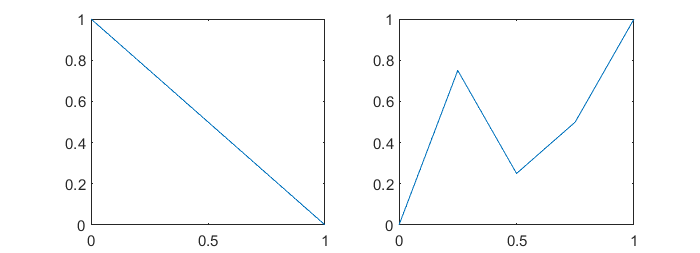
\includegraphics[width=0.8\linewidth]{hw1_1_2}
    \caption{transformation functions. 
    left: coordinates of [0,1], [1,0], right: coordinates of [0 .25 .5 .75 1],[0 .75 .25 .5 1].}
    \label{fig:2}
    \vspace{-2mm}
\end{figure}

\figurename{\ref{fig:2}} plots two transformation functions. It can be seen that left transformation
inverses the input intensity, which is proved on middle version of \figurename{\ref{fig:1}}.
In the rightmost cameraman image, darkest part such as coat is whitened and background, which has relatively
high intensity, is darkened. This corresponds with right function of \figurename{\ref{fig:2}}.  

\begin{figure}[h]
    \centering
    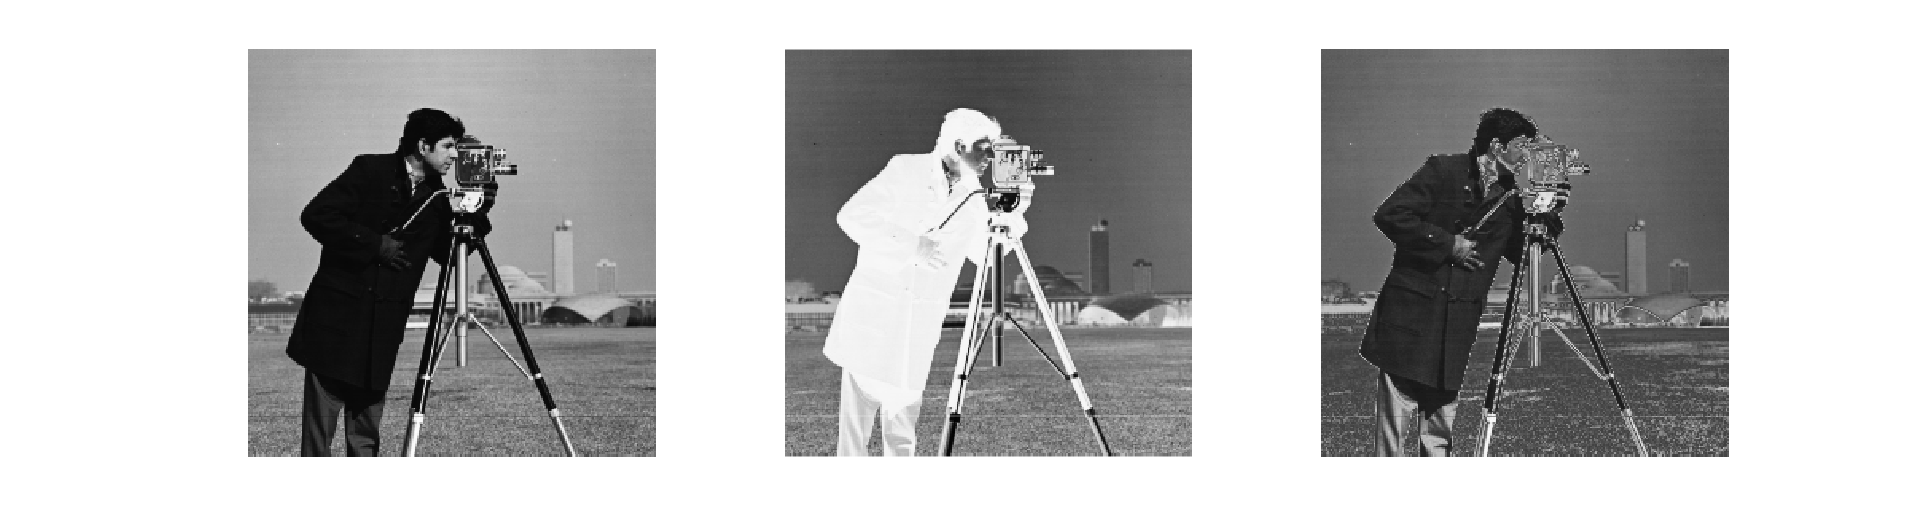
\includegraphics[width=\linewidth]{hw1_1}
    \caption{result of running hw1\_1.m}
    \label{fig:1}
    \vspace{-2mm}
\end{figure}

\section*{Problem 2: Image Histogram}

hw1\_2.m loads input.jpg and plot histogram of the image.
Hist.m implements gathering histogram statistics.
Algorithm\ref{alg:2} is the pseudocode for the file.

\begin{algorithm}
\caption{Hist.m}
\label{alg:2}
\KwIn{$input$ of size $(M,N)$}
$hist = zeros$\;
\For{$i = 1:M$}{
    \For{$j = 1:N$}{
        $hist(input(i,j)) += 1$\;
    }
}
plot $hist$\;
\end{algorithm}

\figurename{\ref{fig:3}} is the result of the hw1\_2.m. It can be seen that majority of the intensities
are concentrated on low range, which can be inferred from the darkness of the image.

\begin{figure}[h]
    \centering
    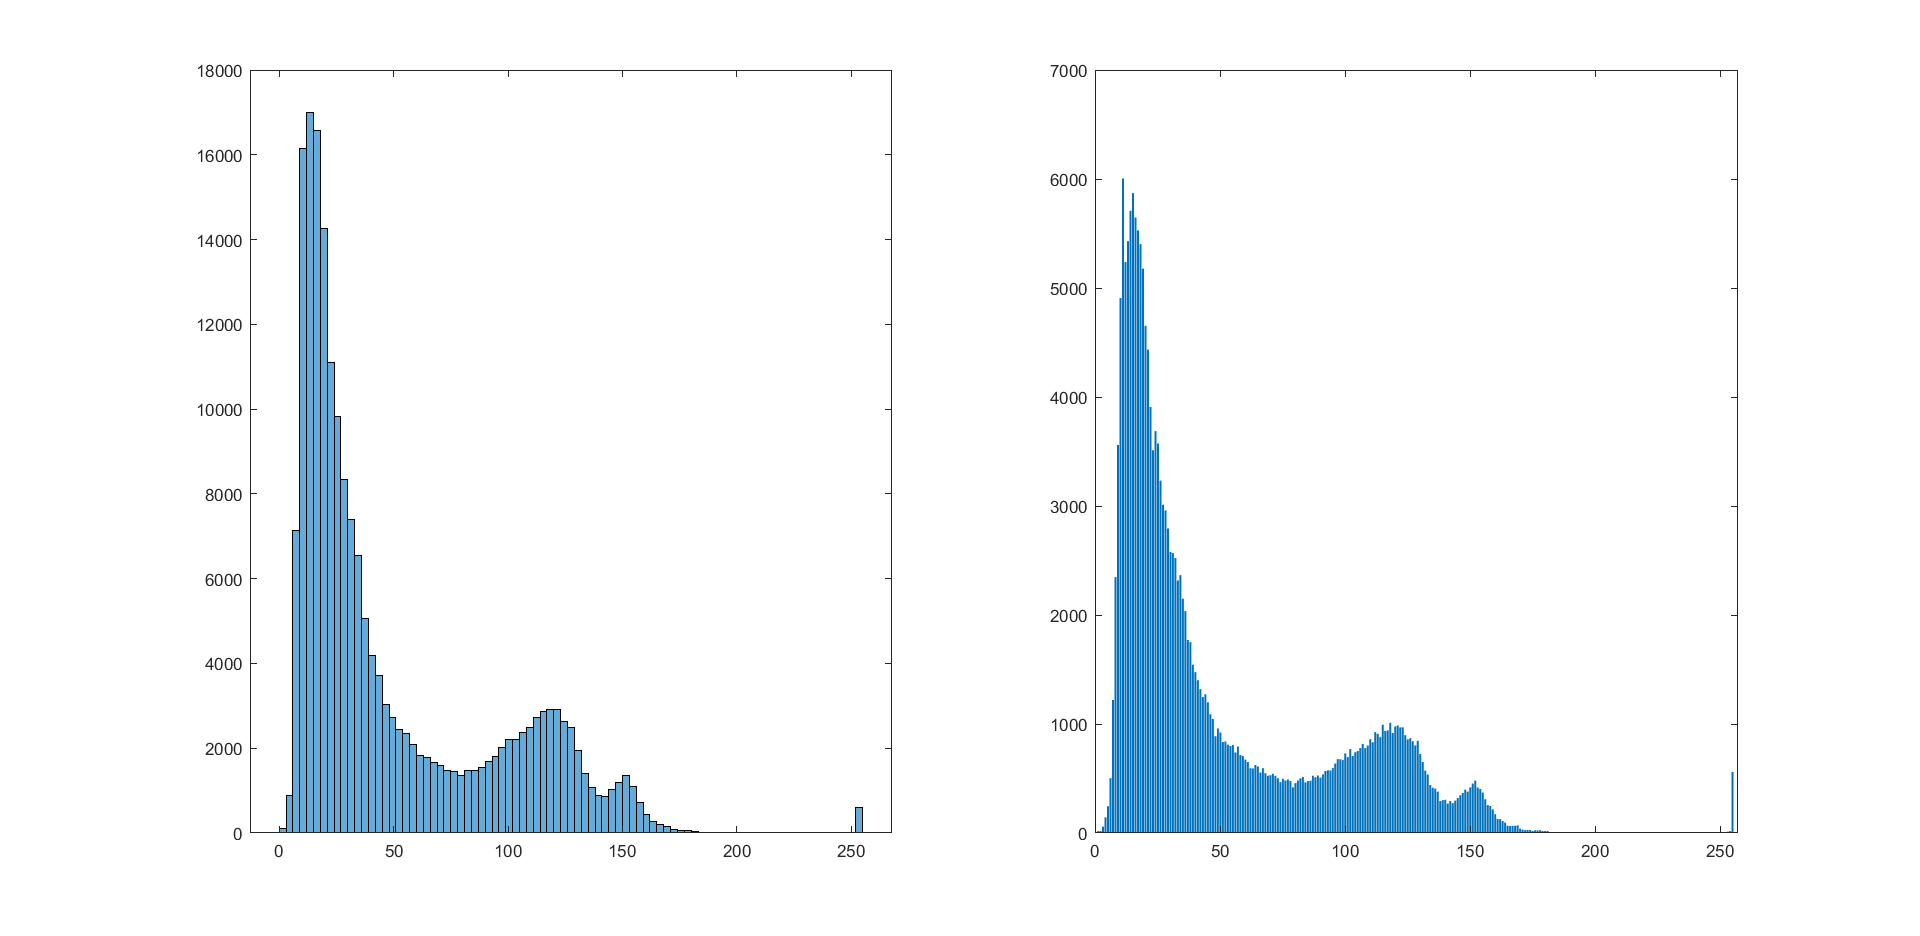
\includegraphics[width=0.6\linewidth]{hw1_2}
    \caption{histogram visualizations.}
    \label{fig:3}
    \vspace{-2mm}
\end{figure}

\section*{Problem 3: Histogram Equalization}

hw1\_3.m loads input.jpg and applies histogram equalization.
HistEq.m accepts input as image and output histogram-equalized version of the image.
The pseudocode for HistEq.m can be found in Algorithm\ref{alg:3}. It internally
build lookup-table(LUT) for intensity transformation.

\begin{algorithm}
\caption{HistEq.m}
\label{alg:3}
\KwIn{$input$ of size $(M,N)$}
\KwOut{$output$}
build histogram $hist$ from $input$\;
$lut = zeros$\;
    
\For{$i = 1:L$}{
    $z = sum(hist(1:i))$\;
    $z = z * (L-1) / (M * N)$\;
    $lut(i) = z$\;
}

$output = input$\;
\For{$i = 1:M$}{
    \For{$j = 1:N$}{
        $output(i,j) = lut(input(i,j))$\;
    }
}
\end{algorithm}

\figurename{\ref{fig:4}} depicts the resulting image and its corresponding histogram. 
It can be seen that the resulting image has enhanced contrast, and the equalized histogram
has more flattened distribution than the original histogram.
Transformed histogram follows more to uniform than the original. 

\begin{figure}[h]
    \centering
    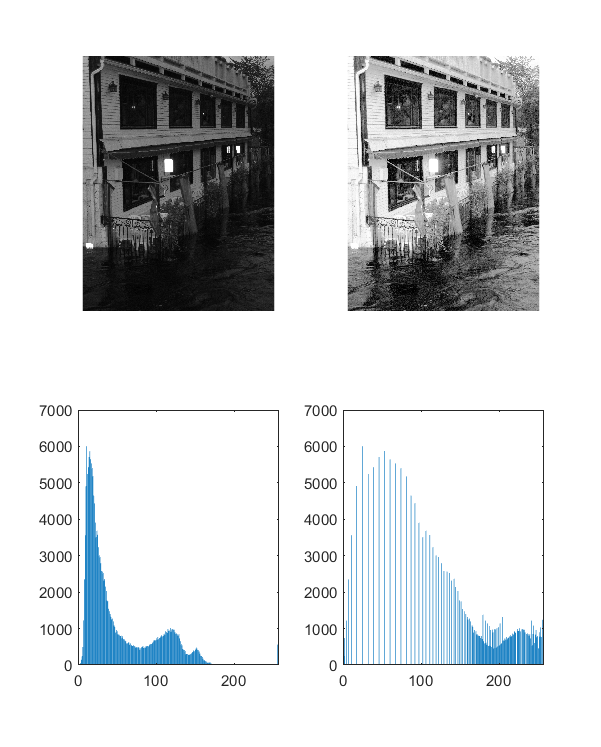
\includegraphics[width=\linewidth]{hw1_3}
    \caption{Result image of histogram equalization and the corresponding histogram.
    left: original image and its histogram, right: histogram-equalized image and its histogram.}
    \label{fig:4}
    \vspace{-2mm}
\end{figure}

\section*{Problem 4: Histogram Equalization}

Histogram equalized image(rightside of \figurename{\ref{fig:4}}) has better 
overall contrast than the original, but some details on lighter part 
is lost due to over-brightness.
To solve the issue, adaptive histogram equalization is implemented in
HistEq\_v2.m. In naive approach, each pixel is equalized base on the histogram
of its neighbors. This requires too much computation complexity, thus
each pixel is interpolated from the neighboring tile histograms.
Detailed implementation is in Algorithm\ref{alg:4}. Detailed corner case 
exceptions are ignored on the pseudocode.

\begin{algorithm}
\caption{HistEq\_v2.m}
\label{alg:4}
\KwIn{$input$, 
$tile\_x$, $tile\_y$: number of tiles in x/y-axis of $input$, 
$tile\_w$, $tile\_h$: width/height of each tile}
\KwOut{$output$}
$hist = zeros$\;
$lut = zeros$\;
\For{$tile\_i = 1:tile\_x$}{
    \For{$tile\_j = 1:tile\_y$}{
        build $lut_i,j$ for $tile_i,j$\;
    }
}
        
$output = input$\;
\For{$i = 1:input\_x$}{
    $tile\_i = floor(i/tile\_w - 0.5)$\;
    $prob\_i = (i/tile\_w - 0.5) - floor(i/tile\_w - 0.5)$\;

    \For{$j = 1:input\_y$}{
        $tile\_j = floor(j/tile\_h - 0.5)$\;
        $prob\_j = (j/tile\_h - 0.5) - floor(j/tile\_h - 0.5)$\;
        \BlankLine
        $output(i,j) = ((lut_{i,j}(input(i,j)) * (1-prob\_j)) +
        (lut_{i,j+1}(input(i,j)) * prob\_j)) * (1-prob\_i) +
        ((lut_{i+1,j}(input(i,j)) * (1-prob\_j)) + 
        (lut_{i+1,j+1}(input(i,j)) * prob\_j)) * prob\_i$\;
    }
}
\end{algorithm}

This gives better visualization than naive histogram equalization in 
\figurename{\ref{fig:6}} (third image). Some details on sidewall of the building is restored,
fence becomes sharper etc. However, some artifacts also arise, make it look like stained.
For further improvement, additional contrast limitation, histogram clipping, is added on the adaptive
histogram equalization(CLAHE, Contrast Limited AHE), implemented on HistEq\_v3.m.

Histogram clipping is done as follows: For given histogram within a tiled
segment, clip the histogram on certain limit and re-distribute the remaining
intensities across the whole intensity range. This limits maximum contrast
amplification, thus reducing the boost effect of noises.

From the fourth image in \figurename{\ref{fig:6}}, it can be seen that 
histogram clipping limits constrast so that the overall image becomes more
natural on one hand and details being boosted on the other.

\begin{figure*}[t]
    \centering
    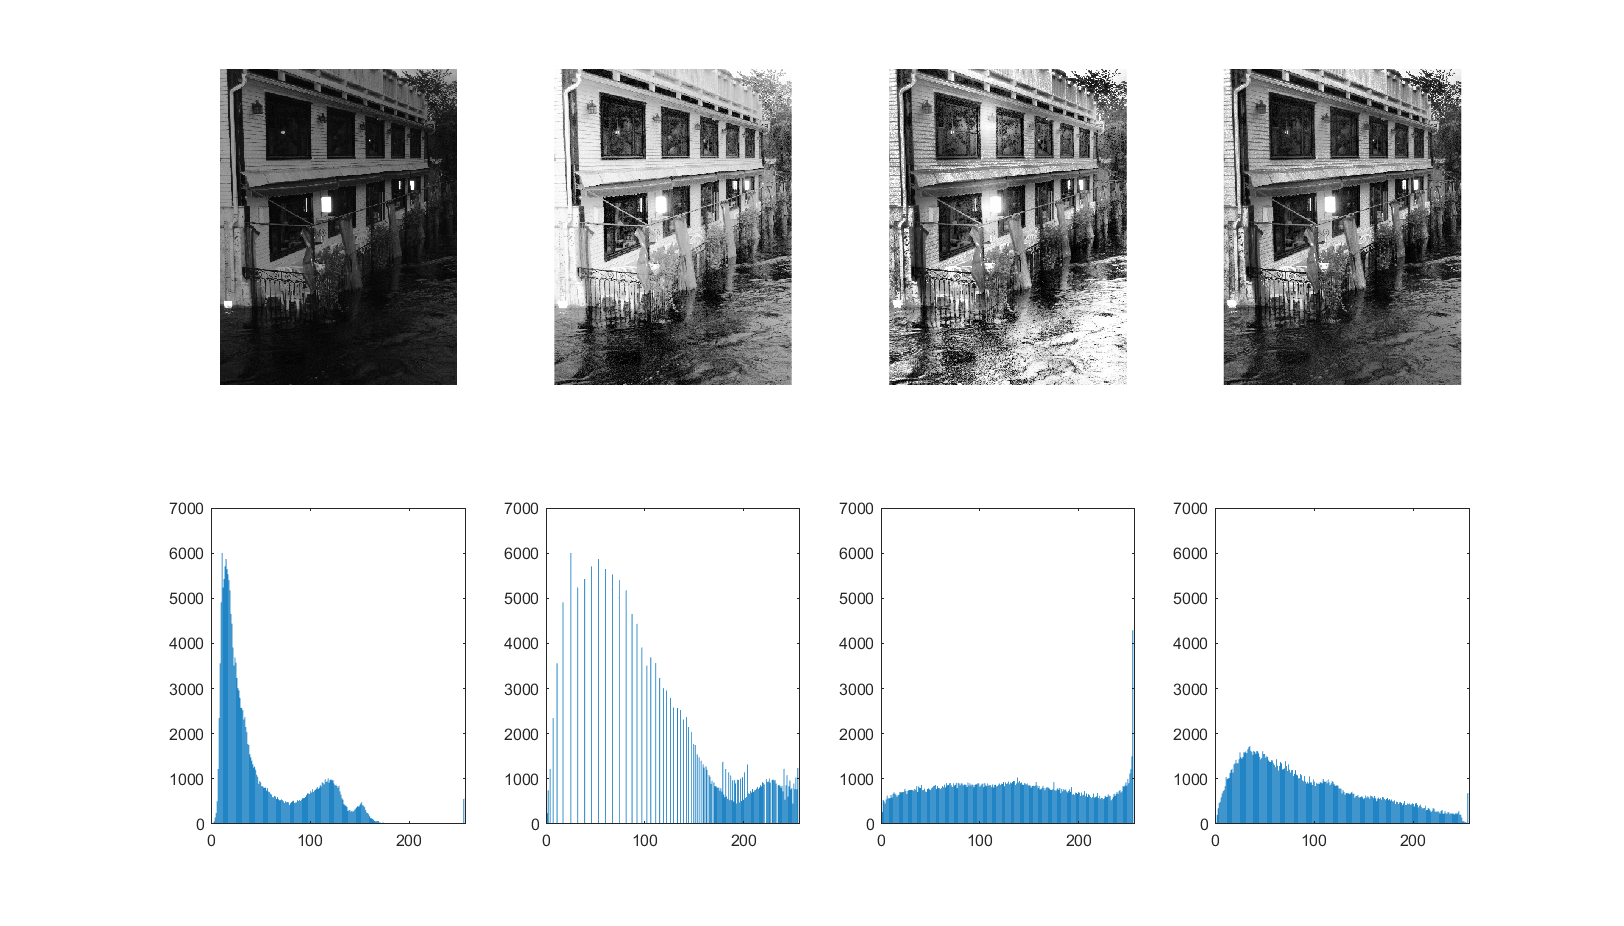
\includegraphics[width=\linewidth]{hw1_4}
    \caption{Results of several histogram equalizations and their histograms. 
    first: original image. second: vanilla histogram equalization.
    third: adaptive histogram equalization(tile size=8x8).
    fourth: contrast limited adaptive histogram equalization(tile size=8x8, clip threshold=4).}
    \label{fig:6}
    \vspace{-2mm}
\end{figure*}

\section*{Problem 5: Histogram Matching}

hw1\_5.m loads input.jpg and performs histogram matching given
target histogram from input\_match.jpg. Histogram matching is done by
applying inverse histogram equalization of input\_match.jpg at histogram-equalized
image from input.jpg. Details can be found in Algorithm\ref{alg:5}.

\begin{algorithm}
\caption{HistMatching.m}
\label{alg:5}
\KwIn{$input$ of size $(M,N)$}
\KwOut{$output$}
build $lut_t$ for historgram equalization given $input$\;
build $lut_g$ for histogram equalization given $input\_match$\;
        
$lut_{g'} = zeros$\;
\For{$i = 1:L$}{
    $lut_{g'}(lut_g(i)) = i$\;
}
\For{$i = 1:L$}{
    \If{$lut_{g'}(i)$ is undefined}{
        assign interpolated value on $lut_{g'}(i)$\;
    }
}
        
$output = input$\;
\For{$i = 1:M$}{
    \For{$j = 1:N$}{
        $output(i,j) = lut_{g'}(lut_t(input(i,j)))$\;
    }
}
\end{algorithm}

When building inverse-LUT from target image, some of the intensities
may be undefined because LUT is not always one-to-one. In that case,
interpolation can be used to predict the missing value.

Result can be found in \figurename{\ref{fig:7}}. The processed image
seems to follow intensity distribution of target image(middle).
Also, the historgam in \figurename{\ref{fig:7}} convinces the
matching be done properly, as the output histogram resembles to the 
target histogram.

\begin{figure*}[h]
    \centering
    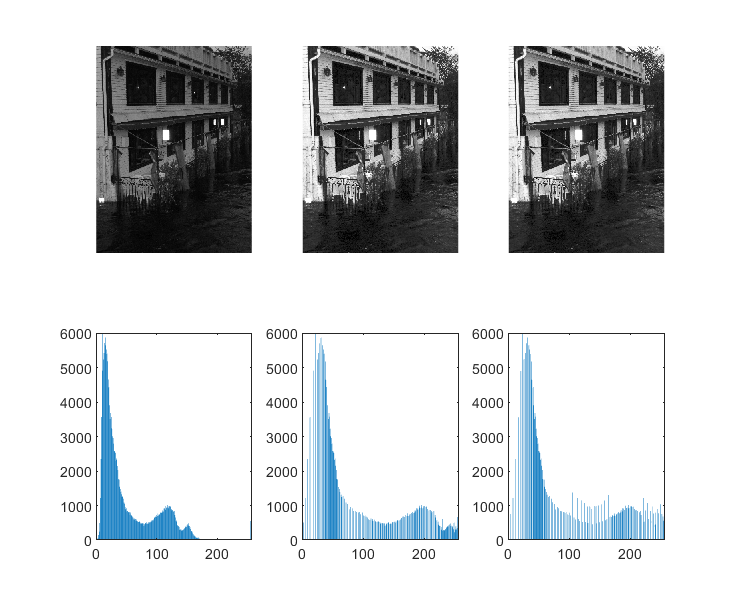
\includegraphics[width=0.7\linewidth]{hw1_5}
    \caption{Result image of histogram matching and its corresponding histogram. 
    left: original image and its histogram. middle: target image and its histogram (target histogram).
    third: result of applying histogram matching on the image and its histogram.}
    \label{fig:7}
    \vspace{-2mm}
\end{figure*}

\end{document}
